\section{Results}\label{sec:results}
We quantify the Jao Gap location along the magnitude axis by first subsampling
our synthetic populations, finding the linear number density along the
magnitude axis of each subsample, averaging these linear number density and
extracting peaks from this above a prominence threshold.w Once we have the peak
location we fit a gaussian to a window centered at the peak giving both an
estimate of the gap location and the gap width. Figure \ref{fig:JaoGapLocator}
shows this fit for both OPAL and OPLIB populations.

Our gap identification method finds two potential gaps in the OPLIB data while
only finding one in the OPAL dataset. 

\begin{figure}
	\centering
	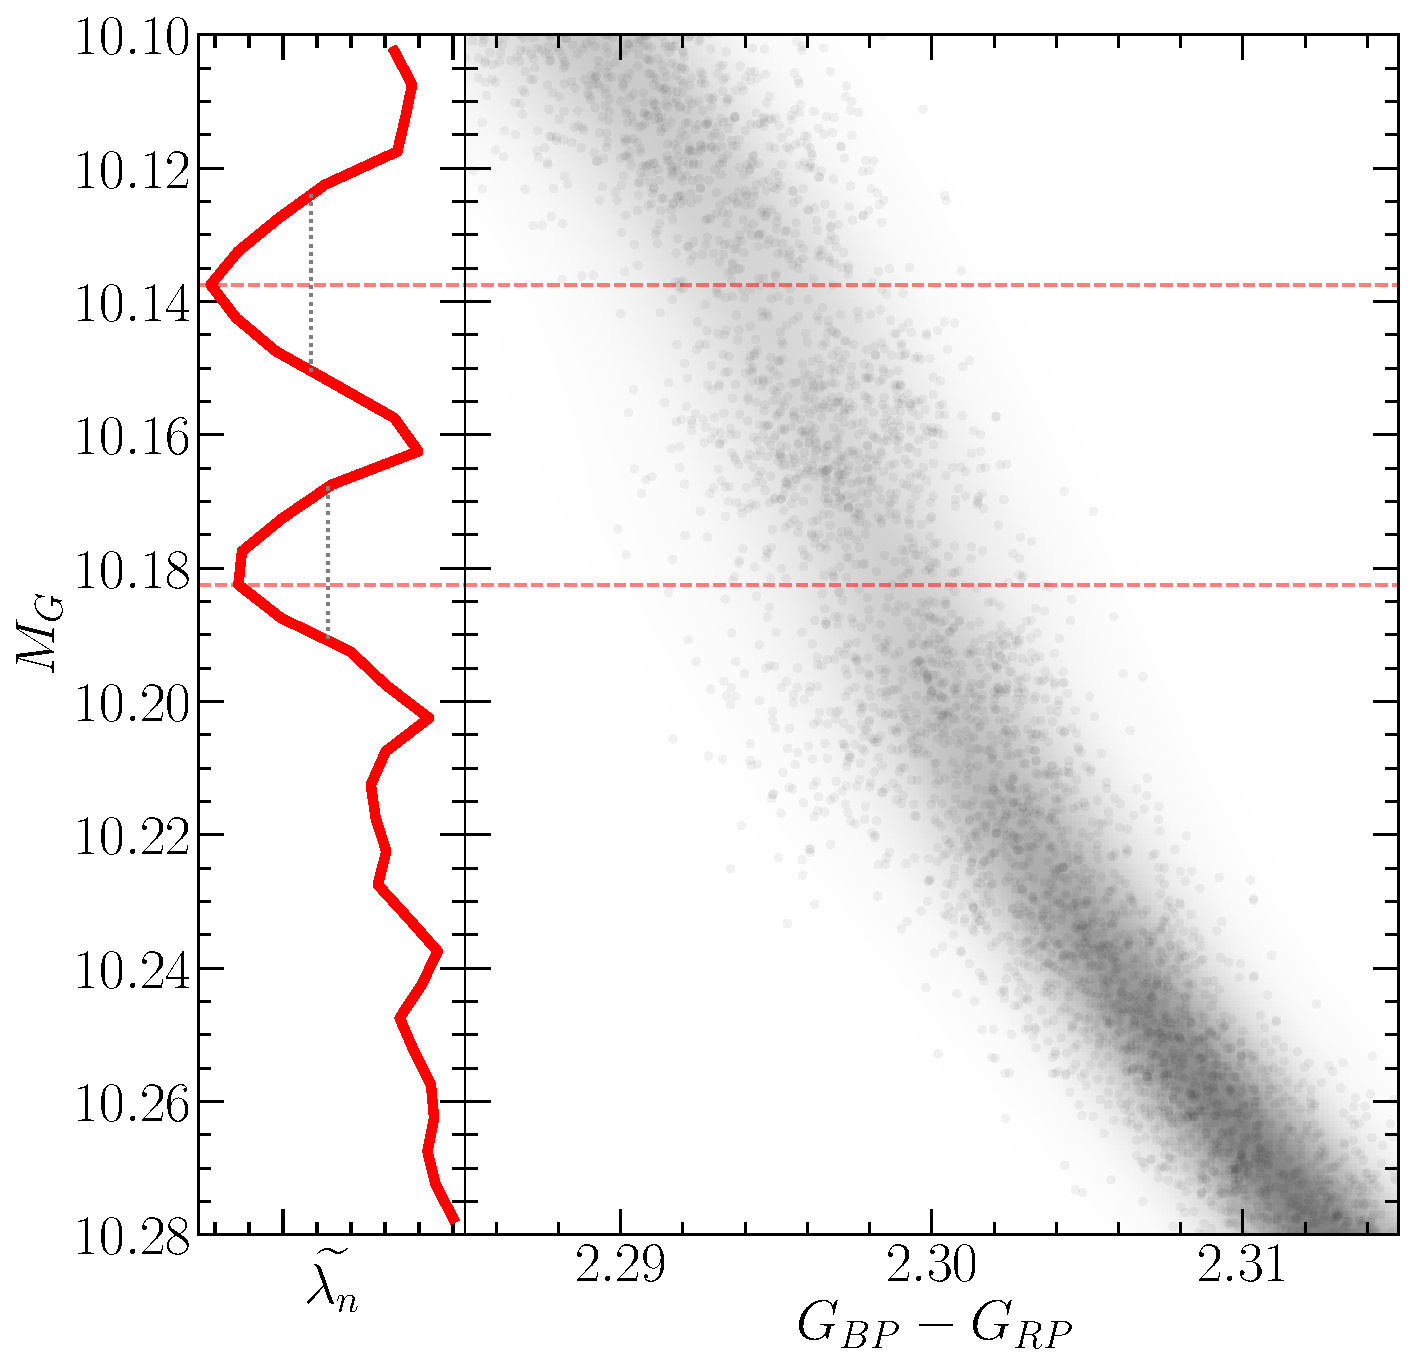
\includegraphics[width=0.45\textwidth]{src/figures/NotebookFigs/OPAL_Jao_locator.png}
	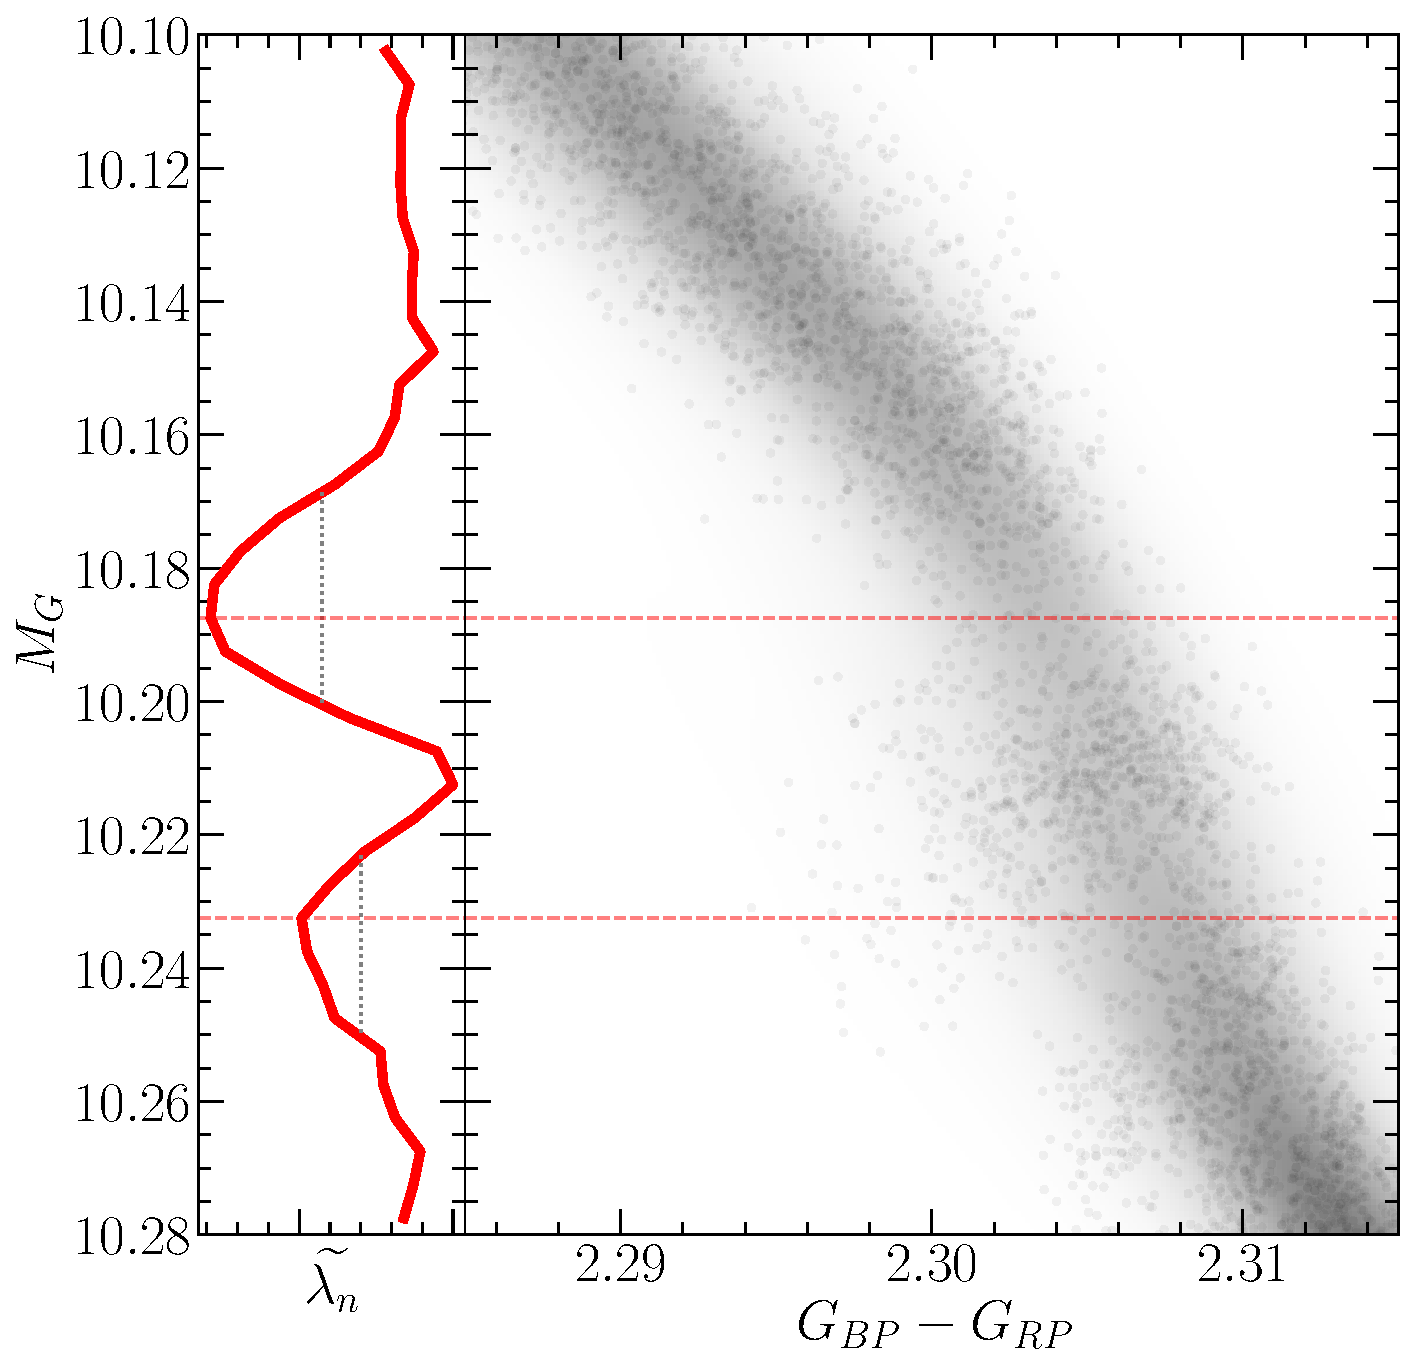
\includegraphics[width=0.45\textwidth]{src/figures/NotebookFigs/OPLIB_Jao_locator.png}
	\caption{(right panels) OPAL (top) and OPLIB (bottom) synthetic
	populations. (left panels) Normalized linear number density along the
	magnitude axis. A dashed line has been extended from the peak through both
	panels to make clear where the Identified Jao Gap location is wrt. to the
	population. }
	\label{fig:JaoGapLocator}
\end{figure}



{\color{red} Talk About results of population synthetis, i.e. where the gap is
in OPAL vs OPLIB, show the CMD}

{\color{red} Then compare the results to observations, comment on which one
matches observations better and also how confident we can be about that}

{\color{red} Comment on if the shift in the gap location is larger or smaller
than the size o fthe gap or the shift due to other effects such as variations
in age or composition, i.e is it Significant enough to matter}

{\color{red} comment on why the gap shifts in the manner which it does, i.e the
opacities are lower. Show how for a constant opacity table increasing the
metallicity (which will also change the opacity) affetcs the gap location)}
